\null\newpage
\section{Hochtöner-Verstärker}\label{sec:4.5}
\subsection{Allgemeines}\label{subsec:4.5.1}
Die gefilterten Hochton-Frequenzen müssen vor dem Abstrahlen verstärkt werden.
Hierfür wird die TDA2030-Grundschaltung(siehe Kapitel \ref{subsec:3.2.2}) verwendet.
Hier ohne Leistungstransistoren, da Hochtöner nicht eine so hohe Leistung ohne Gefahr umsetzen können.
Sie könnten bei zu hoher Leistung durchbrennen, d.h. der Isolierschutzlack der Spule im Lautsprecher wird zu heiß.

\subsection{Zielsetzung}\label{subsec:4.5.2}
Das Eingangssignal soll verstärkt werden um am Ausgang der Schaltung höhere Spannungs-Amplituden und höheren Ströme aufzuweisen. Es soll nach diesem Schritt möglich sein den Hochtöner in einer der zwei Satellitenboxen mit ausreichend Signal zu versorgen, um einen Schalldruck von zumindest Zimmerlautstärke zu erhalten. 
% Sollen wir hier genau das selbe schreiben wie beim TTVerstärker?

\subsection{Schaltung}\label{subsec:4.5.3}
Aus der TDA2030-Grundschaltung (siehe Kapitel \ref{subsec:3.2.2}) folgend ist auch hier ein Spannungsteiler vorgesehen um den Arbeitspunkt einzustellen.
Konkret ist dieser Spannungsteiler aus \enquote{R601} und \enquote{R602} aufgebaut.

\begin{figure} [H]
	\centering	
	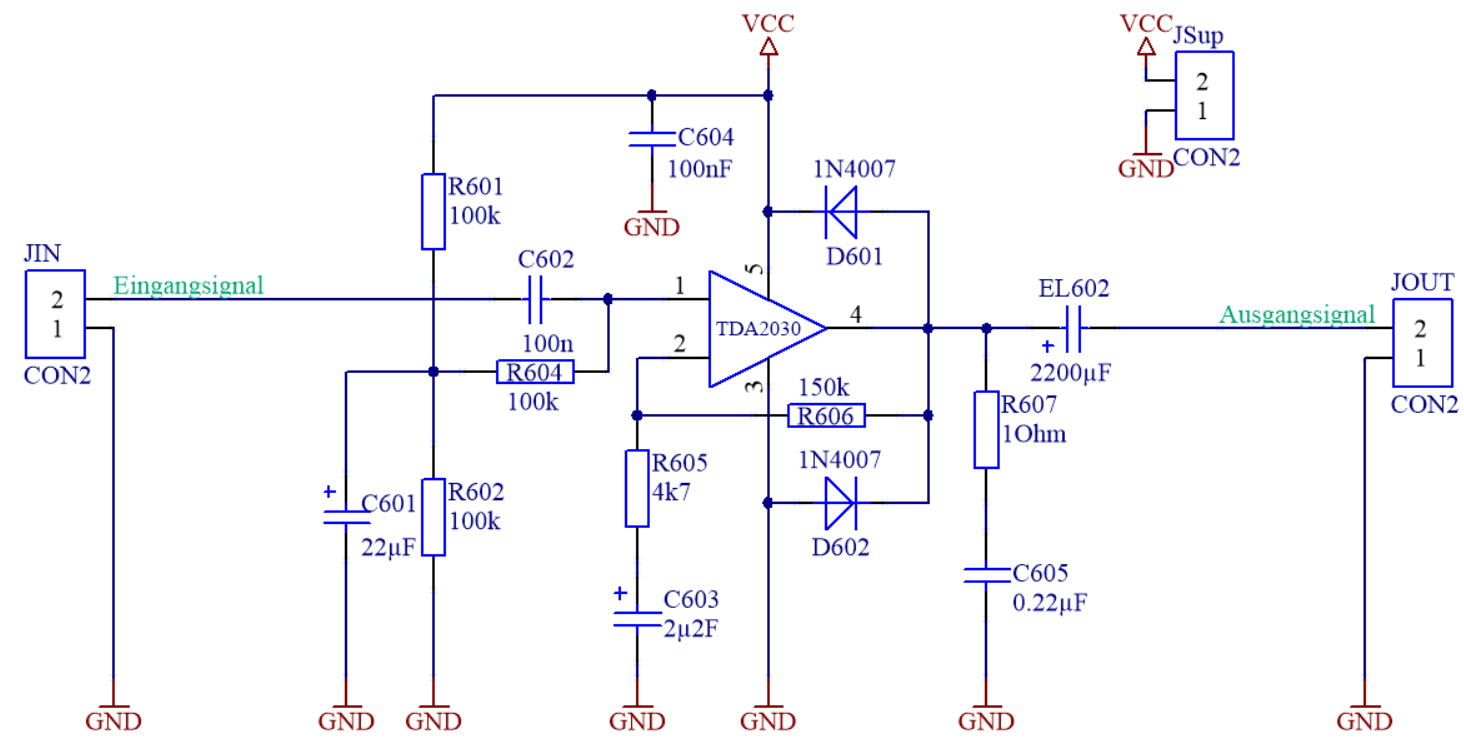
\includegraphics[width=1\textwidth]{img/Print6/HTVerstaerker-Schem.PNG}
	\caption{Hochtöner-Verstärker Schaltung}
	\label {fig:4.5.3.1}
\end{figure}

\subsection{PCB}\label{subsec:4.5.4}
Das Layout wird wieder nach den Grunddesignregeln(siehe Kapitel \ref{subsec:3.1.2}) erstellt.\\
Eine große Fläche über dem TDA2030 wird vorgesehen um einen Testkühlkörper mit dem Print mechanisch verbinden zu können.
Es dient zur Verringerung der Hebelwirkung.
%Mit Fortschreiten der Arbeit wurde die Fläche gekürtzt um mit dem neuen Kühlkörper eben abzuschließen.

\begin{figure} [H]
	\centering	
	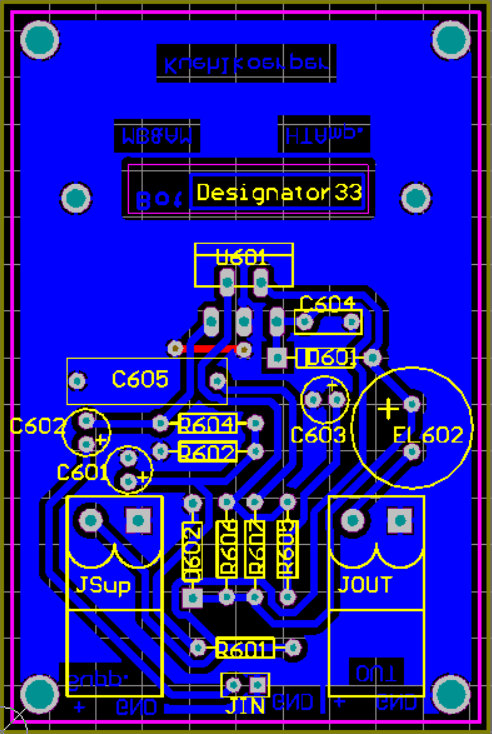
\includegraphics[width=0.7\textwidth]{img/Print6/HTVerstaerker-PCB.PNG}
	\caption{Hochtöner-Verstärker PCB}
	\label {fig:4.5.4.1}
\end{figure}

